\chapter{Results \& discussion}
Eivind the GOAT

\section{Splitting the chain}
A previous masters student also did this. Boom i replicated his results life is good


eivind cut means that it's not the central bond thats cut, but rather one out to the side. This matches Eivinds new code. 


\begin{figure}
    \centering
    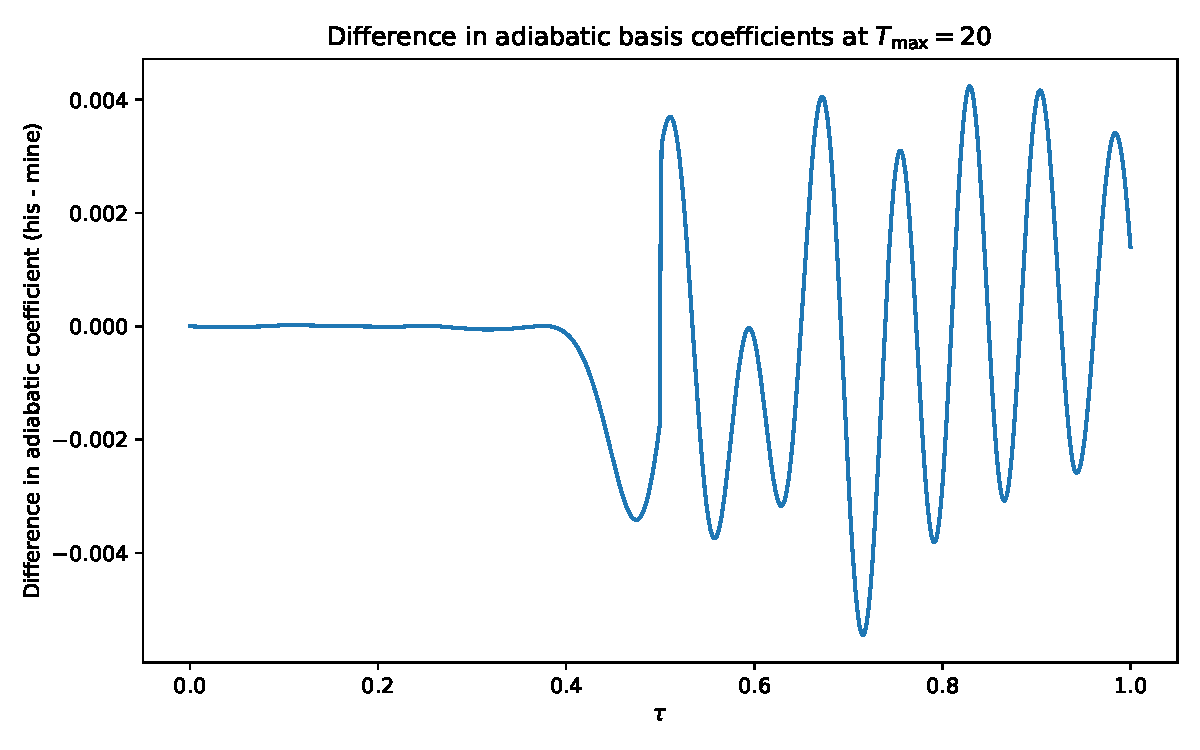
\includegraphics[width = \linewidth]{eivind_cut__trunc=10__eivind_diff_instantaneous_1.pdf}
    \caption{}
    \label{fig:2}
\end{figure}

\begin{figure}
    \centering
    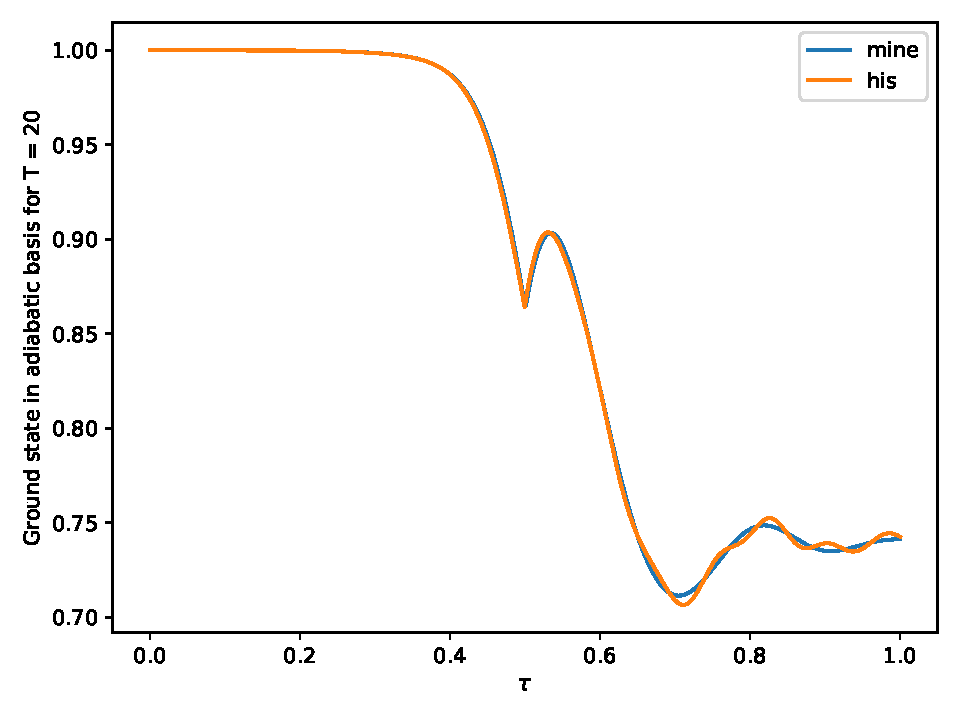
\includegraphics[width = \linewidth]{eivind_cut___eivind_instantaneous_basis.pdf}
    \caption{}
    \label{fig:3}
\end{figure}

\begin{figure}
    \centering
    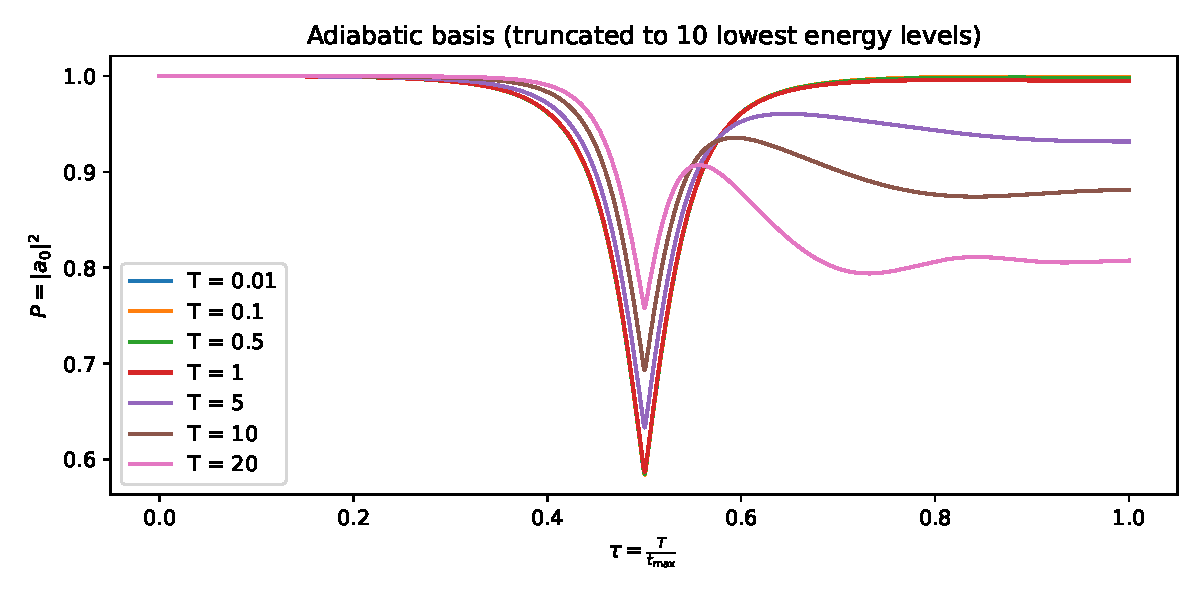
\includegraphics[width = \linewidth]{Proper_cut_chain_cut_chain_trunc=10_7_1.0_2.0_0.5_Adiabatic_precomputed_Kitaev_RK4_N=10_dt=0.001001001001001001_sparse.pdf}
    \caption{}
    \label{fig:4}
\end{figure}

\begin{figure}
    \centering
    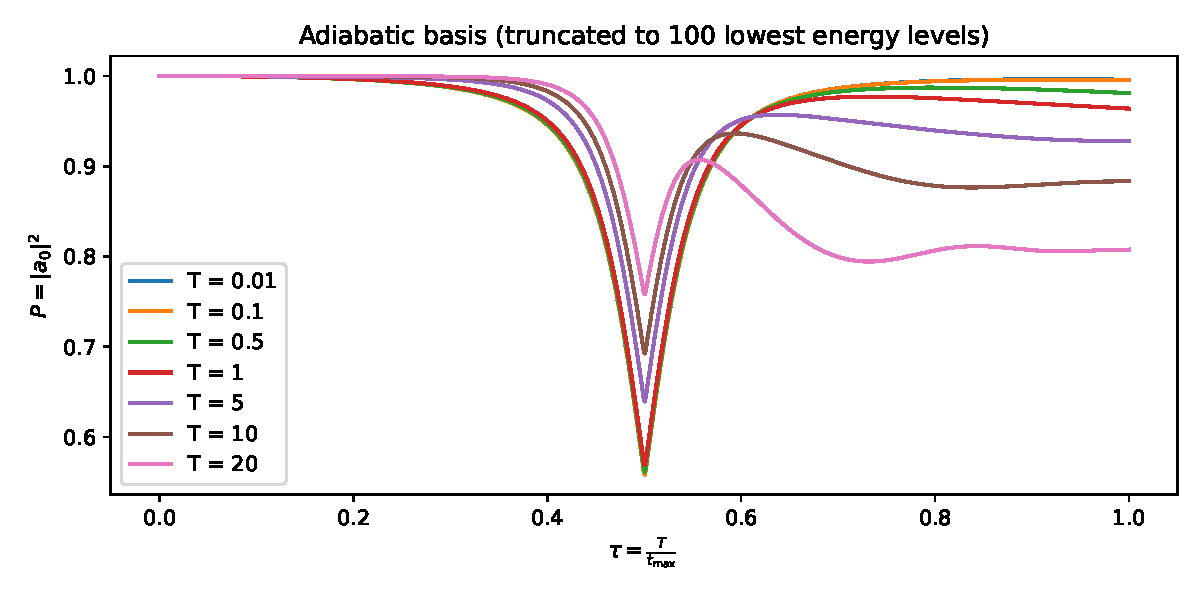
\includegraphics[width = \linewidth]{Proper_cut_chain_cut_chain_trunc=100_7_1.0_2.0_0.5_Adiabatic_precomputed_Kitaev_RK4_N=10_dt=0.001001001001001001_sparse.pdf}
    \caption{}
    \label{fig:5}
\end{figure}



\subsubsection{Schrodinger evolution vs adiabatic evolution}
Time and accuracy wrt truncation

\section{T-junction}
I need a supercomputer :/

\subsection{Pali X-gate}
Exchange 2 and 3

\subsection{Pauli Z-gate}
Exchange 1 and 2 (or 3 and 4)

